% !TeX root = ../Thesis.tex

%************************************************
\chapter{Evaluation}\label{ch:evaluation}
%************************************************
\glsresetall % Resets all acronyms to not used

To answer the main question of this thesis, whether the integration of \glspl{NN} into \gls{VPR} can improve its performance, we optimize and thoroughly evaluate our system.

\section{Evaluation Scenario}

First describing our method of evaluation as well as the specific settings used, we then evaluate the various \gls{NN} candidates against each other to determine the best network structure. Following this, the original \gls{VPR} Placer is evaluated and compared with our versions integrating \glspl{NN}.

\subsection{Selected Benchmarks}\label{ch:benchmarks}

For the final evaluation we select three circuits from the \gls{VPR} benchmark suite that we did not use in any prior part of this project, namely \textit{mcml.blif}, \textit{or1200.blif}, and \textit{diffeq2.blif}. The circuits are selected quasi-randomly, but ensuring that at least each one \textit{big} and one \textit{small} circuit is chosen.

In the same manner we also select an \textit{evaluation} set of one circuit (\textit{raygentop.blif}), which we will need for our chosen method of model selection, detailed in \ref{ch:model-selection}. This set is intentionally small to keep the computational effort of model selection manageable.

As the \gls{VPR} Placement algorithm is a pseudo-randomized heuristic not guarantee to yield reproducible results (when starting from a different state), each evaluation on each of this circuits will be performed with 3 redundant placing attempts with different random seeds to ensure robust results. 

We then select the median of the three performance scores, not their mean, which makes our evaluation robust against outliers.

\subsection{Runtime/Quality Trade-off}

Our metric of choice is runtime/quality trade-off, specifically discretely sampled routing quality (minimum channel width and critical path length) for certain approximate absolute placement run-times. These run-times, or sampling points, are selected per benchmark circuit relative to the runtime of the unchanged \gls{VPR} Placer (t\textsubscript{p}) as:

\begin{itemize}
	\item 1   * t\textsubscript{p}, or \textit{sampling point 1}
	\item 10  * t\textsubscript{p}, or \textit{sampling point 10}
	\item 50  * t\textsubscript{p}, or \textit{sampling point 50}
\end{itemize}

The actual run-time, while not A-Priori \textit{predictable} for a certain configuration of the modified \gls{VPR} Placer, can easily be \textit{controlled} with the \textit{inner\_num} setting of \gls{VPR}.\cite{vtr8} 

Based on observations we state without formal proof that most of the computations of the \gls{VPR} Placer are performed inside each of these steps. Furthermore, while steps perform random actions and can have vastly differing run-time, within a certain \textit{temperature level} steps with different run-times are distributed randomly, and the number of steps per temperature is generally high. Therefore, changing this number of steps will not change the distribution of step run-times within a certain temperature-level, which means their average run-time remains approximately the same. Therefore, changes to the \textit{inner\_num} parameter, which is a linear factor for the actual number of steps performed, affect the total runtime of the modified \gls{VPR} Placer approximately linearly.

By placing a benchmark circuit using a fixed setting for \textit{inner\_num}, we acquire the runtime at this setting. As early experiments showed that the runtime of the \gls{VPR} Placer using \glspl{NN} is one to two orders of magnitude slower than using \gls{HPWL}, this value is set to $0.01*num_blocks^(4/3)$, which equals one hundredth of the default value of the \gls{VPR} Placer. Therefore, this first check is estimated to take approximately as much time as the unchanged \gls{VPR} at sampling point 1.

Now, \textit{inner\_num} can be scaled appropriately to gain quality scores at each sampling point.

Evaluating the performance of a certain \gls{NN} during model selection consists of the following steps:

\begin{itemize}
	\item integration into \gls{VPR}
	\item determining the runtime over \textit{inner\_num}
	\item setting \textit{inner\_num} appropriately for sampling point 10
	\item placing the evaluation circuit three times
	\item routing each placement and logging average quality 
\end{itemize}

The final evaluation of the best \gls{CNN} and \gls{RNN} against unchanged \gls{VPR} is performed as follows:

\begin{itemize}
	\item integration into \gls{VPR}
	\item determining the runtime over \textit{inner\_num}
	\item setting \textit{inner\_num} appropriately for sampling point 1
	\item placing the test circuits three times
	\item routing each placement and logging average quality per circuit
	\item repeating for sampling point 10 and sampling point 50
\end{itemize}

The thus computed quality/runtime trade-off is then compared with that of the unchanged \gls{VPR} Placer.

The \gls{VPR} Router primarily optimizes the \textit{channel width}, or maximum number of parallel routing channels used by the routing, by determining the minimum routable value via binary search. Therefore we select \textit{channel width} as the primary evaluation metric. In the final evaluation we will, however, also compare critical path lengths, as this, as \gls{VPR}'s secondary optimization target, defines the maximum operateable frequency of the circuit, directly influencing its computational capabilities.

\section{Model Selection}\label{ch:model-selection}

Although \glspl{NN} automatically tune their parameters to fit the target function, the structure and properties of the network itself has to be specified explicitly. While recent works try to automate even this, it is usually still necessary to manually design networks to achieve good results.

During model selection, \glspl{CNN} and \glspl{RNN} are evaluated independently from each other and using the same methodology. This yields a best \gls{CNN} and a best \gls{RNN}, which will both again be integrated into \gls{VPR} and evaluated against the unchanged Placer.  

\subsection{Empirical Model Search}

Typically, a first working design is found empirically through experimentation, based largely on best practices, related works, and intuition. In our case, the strict requirements on the runtime of the networks restricted the search space considerably, and the model candidates described in \ref{ch:cnn-design} and \ref{ch:rnn-design} represent the obvious choices for small and simple networks.

From these candidates, the best one is selected by evaluating each independently on evaluation data different from the training and the final test data, and comparing the results.

\subsection{\gls{HPO}}

\begin{figure}
	\begin{subfigure}[b]{0.45\linewidth}
		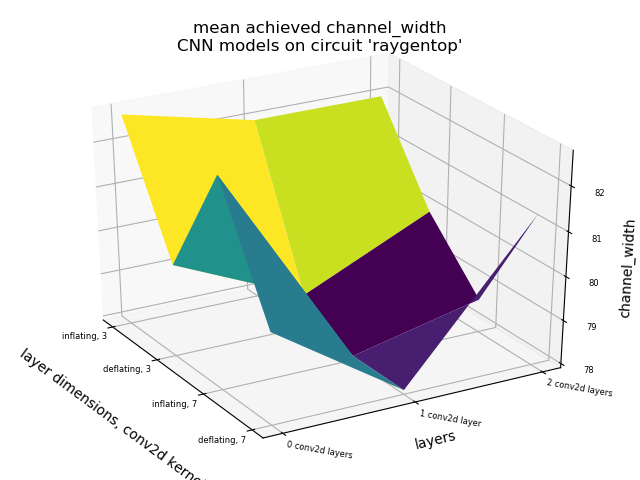
\includegraphics[width=\linewidth]{plots/cnn-hyperopt-chan-width.png}
		\caption{\glspl{CNN} - channel width}
	\end{subfigure}
	\begin{subfigure}[b]{0.45\linewidth}
		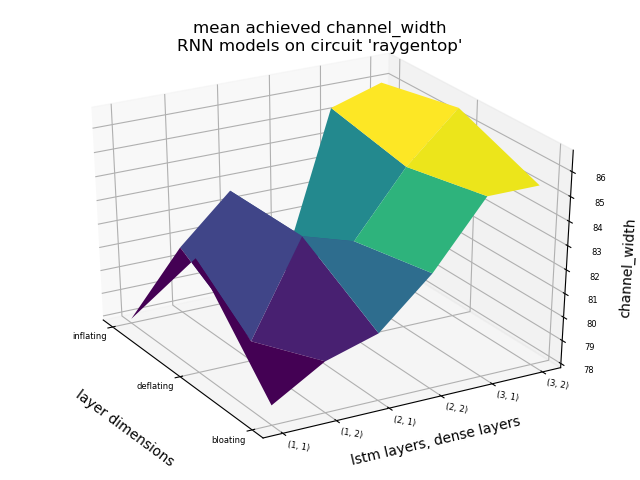
\includegraphics[width=\linewidth]{plots/rnn-hyperopt-chan-width.png}
		\caption{\glspl{RNN} - channel width}
	\end{subfigure}
	\begin{subfigure}[b]{0.45\linewidth}
		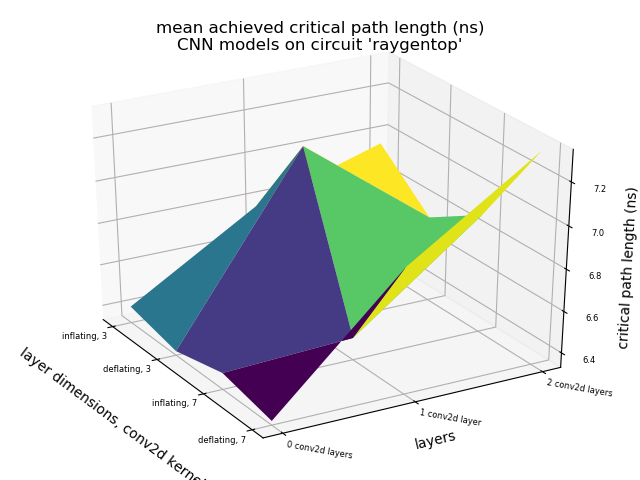
\includegraphics[width=\linewidth]{plots/cnn-hyperopt-critical-path.png}
		\caption{\glspl{CNN} - critical path length}
	\end{subfigure}
	\begin{subfigure}[b]{0.45\linewidth}
		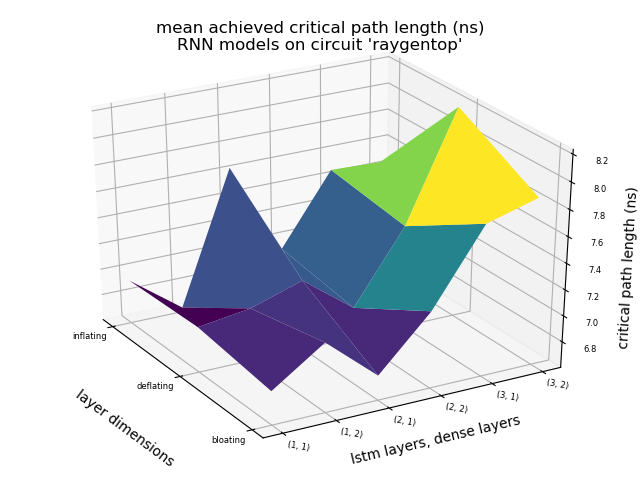
\includegraphics[width=\linewidth]{plots/rnn-hyperopt-critical-path.png}
		\caption{\glspl{RNN} - critical path length}
	\end{subfigure}
	\caption{Achieved performance over model configurations.}
	\label{fig:eval-hyperopt-surface}
\end{figure}

As these groups of candidates are generated from discrete parameters, e.g. dense layer count, this model selection approach constitutes a grid search over these hyperparameters.

By evaluating the \gls{NN} candidates on the evaluation set at sampling point 10 we determine their relative performance. A visualization of the results in Figure \ref{fig:eval-hyperopt-surface} clearly shows a correlation between network complexity and routing quality: Smaller networks produce better results, with the exception of \glspl{CNN} without convolutional layers. These models, using less time for a prediction, allow for a higher number of moves per temperature step, although producing less accurate predictions than their more complex counterparts. The properties of convolutional layers, while computationally being rather expensive (at least compared to the "tiny" dense layers), seem to be beneficial to accurately predict the wiring cost. As the \gls{LSTM} layers of the \glspl{RNN} are required to encode the input data for the following dense layers, their suitedness to the problem can not be measured that easily.

\begin{table}
	\begin{tabular}{lllrr}
		\toprule
		&           &   &  channel\_width &  critical\_path \\
		conv\_layer & structure & kernel &                &                   \\
		count &  & size &                &                   \\
		\midrule
		0 & deflating & -1 &      80.000000 &          6.349267 \\
		& inflating & -1 &      82.666667 &          6.408450 \\
		1 & deflating & 3 &      78.666667 &          7.193833 \\
		&           & 7 &      78.000000 &          6.928623 \\
		& inflating & 3 &      82.000000 &          6.771453 \\
		&           & 7 &      78.000000 &          6.435523 \\
		2 & deflating & 3 &      80.000000 &          6.736223 \\
		&           & 7 &      81.333333 &          7.324657 \\
		& inflating & 3 &      82.000000 &          6.955660 \\
		&           & 7 &      78.666667 &          6.892683 \\
		\bottomrule
	\end{tabular}
	\caption{Results of \gls{CNN} HPO. TODO update values}
	\label{table:cnn-hyperopt-results}
\end{table}

\begin{table}
	\begin{tabular}{lllrr}
		\toprule
		&   &           &  channel\_width &  critical\_path \\
		lstm\_layer & dense\_layer & structure &                &                   \\
		count & count &  &                &                   \\
		\midrule
		1 & 1 & bloating &          78.67 &              6.86 \\
		&   & deflating &          82.67 &              6.95 \\
		&   & inflating &          78.00 &              6.93 \\
		& 2 & bloating &          80.00 &              7.13 \\
		&   & deflating &          78.67 &              7.01 \\
		&   & inflating &          80.67 &              6.63 \\
		2 & 1 & bloating &          80.67 &              6.79 \\
		&   & deflating &          82.67 &              7.13 \\
		&   & inflating &          82.67 &              7.65 \\
		& 2 & bloating &          82.67 &              7.19 \\
		&   & deflating &          82.00 &              6.83 \\
		&   & inflating &          78.67 &              6.93 \\
		3 & 1 & bloating &          85.33 &              7.76 \\
		&   & deflating &          84.67 &              7.38 \\
		&   & inflating &          85.33 &              7.48 \\
		& 2 & bloating &          85.33 &              7.86 \\
		&   & deflating &          86.67 &              8.20 \\
		&   & inflating &          86.00 &              7.46 \\
		\bottomrule
	\end{tabular}
	\caption{Results of \gls{RNN} HPO. TODO update values}
	\label{table:rnn-hyperopt-results}
\end{table}

The exact results are presented in \ref{table:cnn-hyperopt-results} and \ref{table:rnn-hyperopt-results}. We thus select \textit{1\_conv\_layers\_deflating\_kernel\_size\_7} and \textit{1\_lstm\_layers\_1\_dense\_layers\_inflating} as the best \gls{CNN} and \gls{RNN} models, respectively.

\begin{figure}
	\begin{subfigure}[b]{0.45\linewidth}
		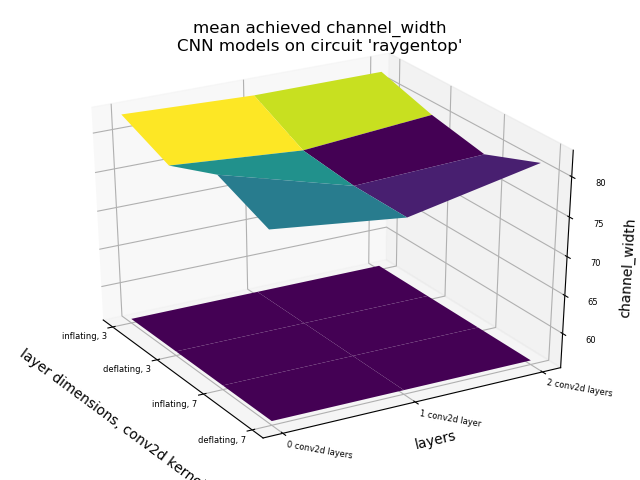
\includegraphics[width=\linewidth]{plots/cnn-hyperopt-chan-width-with-reference.png}
		\caption{\glspl{CNN} - channel width}
	\end{subfigure}
	\begin{subfigure}[b]{0.45\linewidth}
		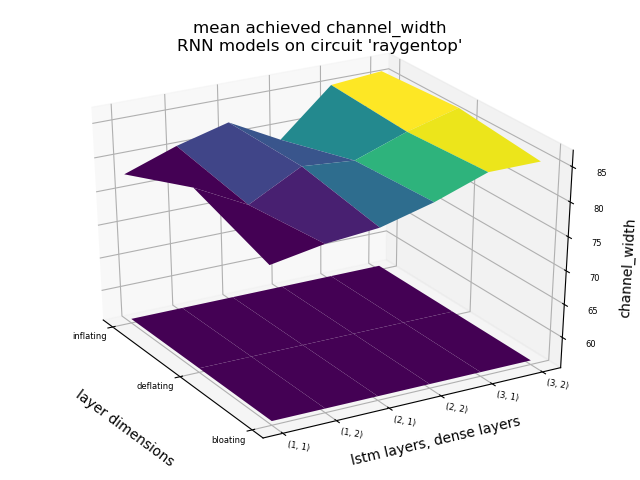
\includegraphics[width=\linewidth]{plots/rnn-hyperopt-chan-width-with-reference.png}
		\caption{\glspl{RNN} - channel width}
	\end{subfigure}
	\begin{subfigure}[b]{0.45\linewidth}
		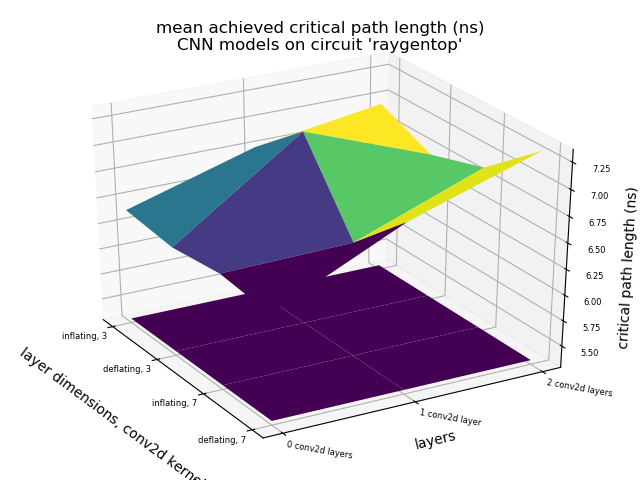
\includegraphics[width=\linewidth]{plots/cnn-hyperopt-critical-path-with-reference.png}
		\caption{\glspl{CNN} - critical path length}
	\end{subfigure}
	\begin{subfigure}[b]{0.45\linewidth}
		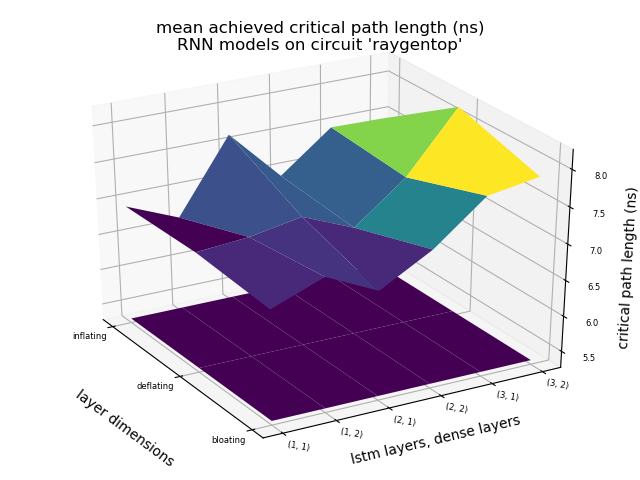
\includegraphics[width=\linewidth]{plots/rnn-hyperopt-critical-path-with-reference.png}
		\caption{\glspl{RNN} - critical path length}
	\end{subfigure}
	\caption{Achieved performance over model configurations with performance of reference system.}
	\label{fig:eval-hyperopt-surface-reference}
\end{figure}

By comparing the performance to that of the unchanged \gls{VPR} Placer we can, however, also see, that none of the \glspl{NN} is able to beat \gls{HPWL} at sampling point 10 (see Figure \ref{fig:eval-hyperopt-surface-reference}).

\section{Results}

With a single network per type the modified \gls{VPR} Placer can now be evaluated against the unchanged version (reference system).

\begin{figure}
	\centering
	\begin{subfigure}[b]{0.45\linewidth}
		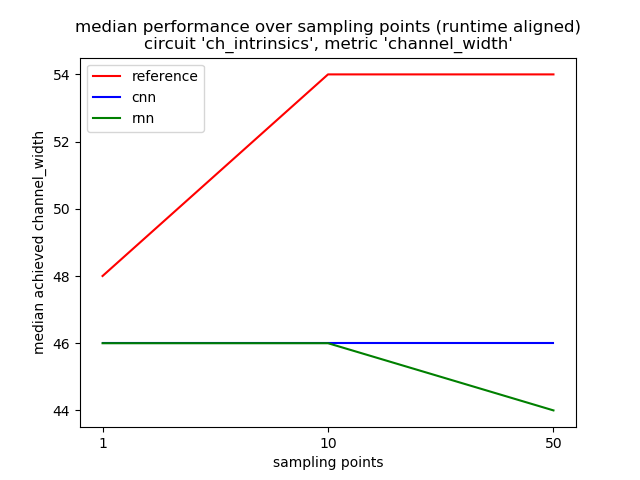
\includegraphics[width=\linewidth]{plots/eval-ch_intrinsics-chan-width-median.png}
	\end{subfigure}
	\begin{subfigure}[b]{0.45\linewidth}
		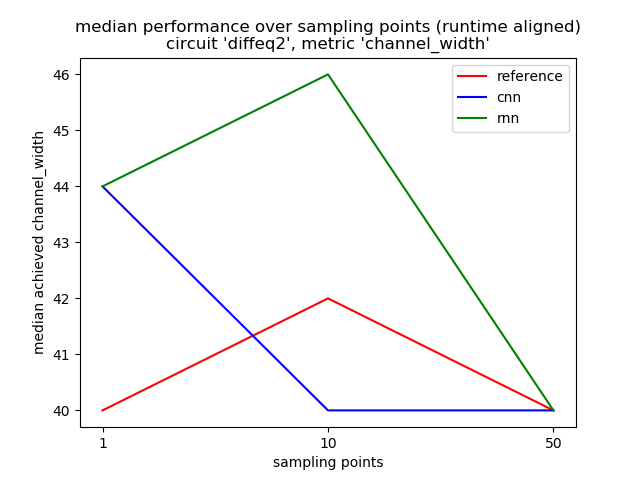
\includegraphics[width=\linewidth]{plots/eval-diffeq2-chan-width-median.png}
	\end{subfigure}
	\begin{subfigure}[b]{0.45\linewidth}
		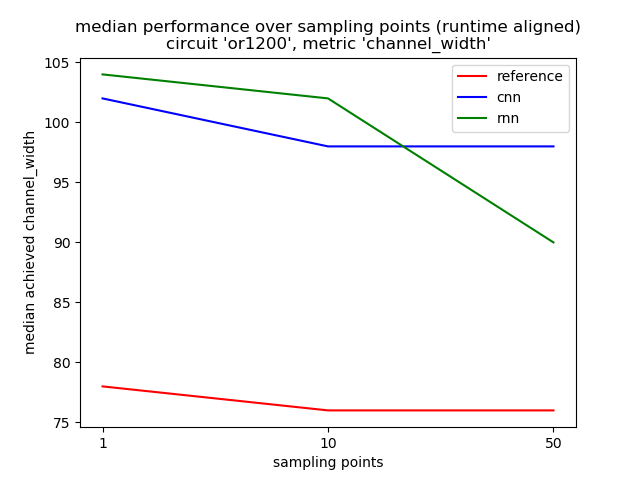
\includegraphics[width=\linewidth]{plots/eval-or1200-chan-width-median.png}
	\end{subfigure}
	\begin{subfigure}[b]{0.45\linewidth}
		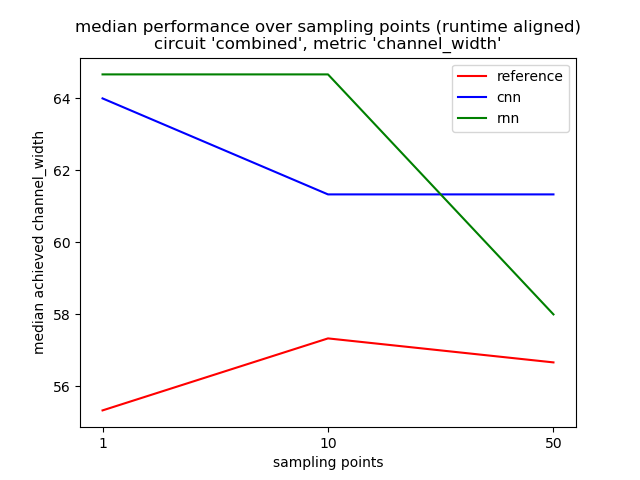
\includegraphics[width=\linewidth]{plots/eval-combined-chan-width-median.png}
	\end{subfigure}
	\caption{Median of achieved channel widths over sampling points per circuit.}
	\label{fig:eval-chan-width-median}
\end{figure}

Figure \ref{fig:eval-chan-width-median} shows the achieved channel widths for the reference system and our \gls{CNN} and \gls{RNN} versions on the test set. Our modified placer using \glspl{NN} is able to significantly outperform the reference system on one of the small circuits and manages to beat it on the other (left), but is inferior on the larger one (top right). 

When combining the results on all three circuits with equal weights, still had higher performance overall, as the "small" improvements on the smaller circuits are drowned out by the huge decrease on the larger one. However, even being able to perform better on \textit{some} circuits can be seen as an improvement, as placing with both the modified and the reference system and taking the better result is also a viable option.

What's more, we can see a clear downward trend in the \gls{RNN} quality/runtime trade-off, which could imply its performance relative to the reference system might increase further beyond the domain we evaluated, i.e. for larger sampling points.

\begin{figure}
	\centering
	\begin{subfigure}[b]{0.45\linewidth}
		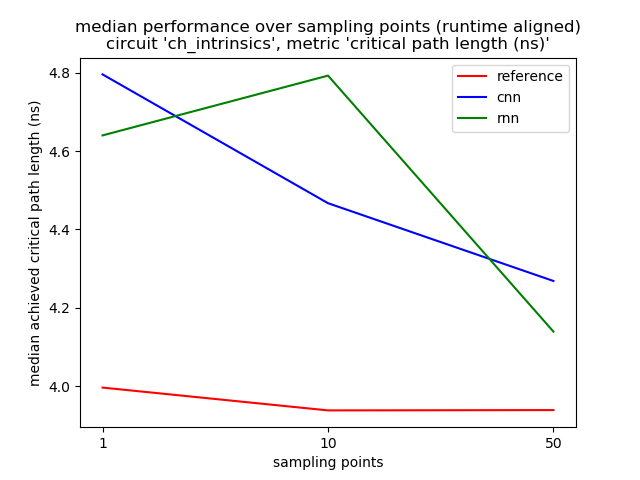
\includegraphics[width=\linewidth]{plots/eval-ch_intrinsics-critical-path-median.png}
	\end{subfigure}
	\begin{subfigure}[b]{0.45\linewidth}
		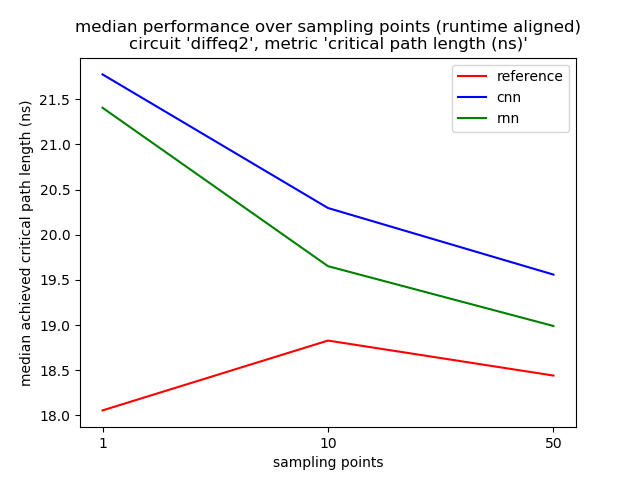
\includegraphics[width=\linewidth]{plots/eval-diffeq2-critical-path-median.png}
	\end{subfigure}
	\begin{subfigure}[b]{0.45\linewidth}
		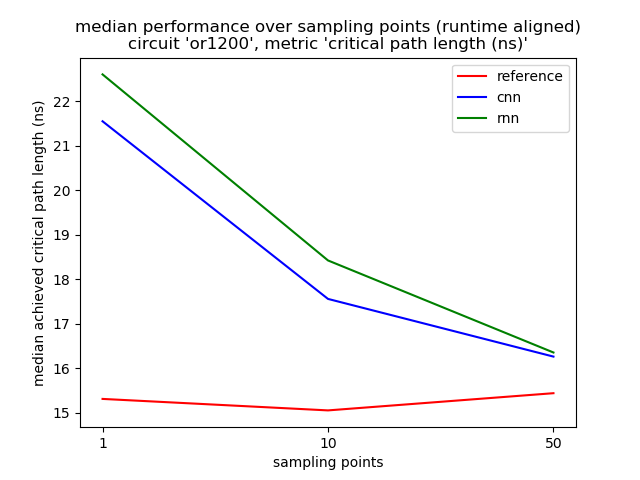
\includegraphics[width=\linewidth]{plots/eval-or1200-critical-path-median.png}
	\end{subfigure}
	\begin{subfigure}[b]{0.45\linewidth}
		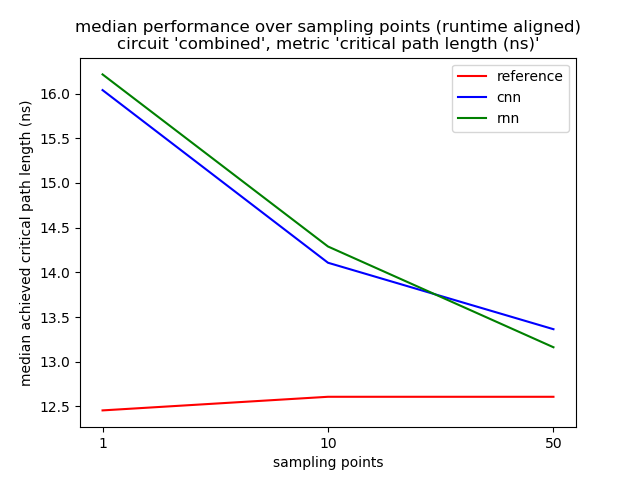
\includegraphics[width=\linewidth]{plots/eval-combined-critical-path-median.png}
	\end{subfigure}
	\caption{Median of achieved channel widths over sampling points per circuit.}
	\label{fig:eval-critical-path-median}
\end{figure}

Inspecting the achieved critical path lengths (Figure \ref{fig:eval-critical-path-median}) further strengthens this hypothesis, exhibiting a significantly steeper downward slope than that of the reference system.

One can also observe that while the \gls{CNN} version initially always beats the \gls{RNN} version, the performance difference clearly diminishes on higher sampling points, and the \gls{RNN} version always wins at the highest tested sampling point.

Therefore we come to the conclusion that the quality/runtime trade-off of the \gls{RNN} version is clearly better than that of the \gls{CNN} version, and thus the \gls{RNN} version is the superior modified system.

With respect to critical path length, the reference system clearly beats both our modified versions on all test circuits and at all sampling points. As the \gls{RNN} version, however, has the runtime/quality trade-off with the steeper slope, both for critical path length and channel width, it seems likely that it indeed constitutes an improvement over the reference system.

\begin{table}
\resizebox{\textwidth}{!}{
\begin{tabular}{lllrrrrrrrr}
	\toprule
	&    & metric & \multicolumn{4}{l}{channel\_width} & \multicolumn{4}{l}{critical\_path} \\
	&    & attempt &             1 &      2 &      3 &     avg &             1 &      2 &      3 &    avg \\
	circuit & sampling & type &               &        &        &         &               &        &        &        \\
		    & point	   & 	  &               &        &        &         &               &        &        &        \\
	\midrule
	diffeq2 & 1  & reference &          40.0 &   40.0 &   40.0 &   40.00 &         18.35 &  18.00 &  18.05 &  18.14 \\
	&    & rnn &          40.0 &   46.0 &   44.0 &   43.33 &         21.73 &  21.24 &  21.40 &  21.46 \\
	&    & cnn &          44.0 &   44.0 &   42.0 &   43.33 &         20.08 &  21.77 &  21.98 &  21.28 \\
	& 10 & reference &          56.0 &   38.0 &   42.0 &   45.33 &         18.83 &  18.98 &  18.51 &  18.77 \\
	&    & rnn &          40.0 &   46.0 &   46.0 &   44.00 &         20.40 &  19.65 &  19.46 &  19.83 \\
	&    & cnn &          42.0 &   40.0 &   38.0 &   40.00 &         21.14 &  20.30 &  19.90 &  20.44 \\
	& 50 & reference &          40.0 &   40.0 &   42.0 &   40.67 &         18.60 &  18.13 &  18.44 &  18.39 \\
	&    & rnn &          46.0 &   40.0 &   40.0 &   42.00 &         20.23 &  18.99 &  18.17 &  19.13 \\
	&    & cnn &          40.0 &   40.0 &   38.0 &   39.33 &         19.48 &  19.56 &  19.68 &  19.57 \\
	or1200 & 1  & reference &          76.0 &   78.0 &   78.0 &   77.33 &         15.32 &  15.50 &  15.18 &  15.33 \\
	&    & rnn &         104.0 &  106.0 &  104.0 &  104.67 &         22.60 &  22.55 &  23.07 &  22.74 \\
	&    & cnn &         106.0 &  102.0 &  102.0 &  103.33 &         20.87 &  23.50 &  21.55 &  21.97 \\
	& 10 & reference &          76.0 &   80.0 &   76.0 &   77.33 &         15.06 &  14.92 &  15.20 &  15.06 \\
	&    & rnn &         106.0 &  100.0 &  102.0 &  102.67 &         19.46 &  18.42 &  17.82 &  18.57 \\
	&    & cnn &          94.0 &   98.0 &  100.0 &   97.33 &         18.28 &  17.07 &  17.56 &  17.64 \\
	& 50 & reference &          76.0 &   78.0 &   74.0 &   76.00 &         15.44 &  15.22 &  15.63 &  15.43 \\
	&    & rnn &          98.0 &   90.0 &   90.0 &   92.67 &         17.16 &  16.34 &  16.36 &  16.62 \\
	&    & cnn &          98.0 &   94.0 &  100.0 &   97.33 &         16.27 &  16.39 &  16.17 &  16.27 \\
	ch\_intrinsics & 1  & reference &          54.0 &   48.0 &   46.0 &   49.33 &          3.94 &   4.00 &   4.64 &   4.19 \\
	&    & rnn &          46.0 &   46.0 &   48.0 &   46.67 &          4.24 &   5.88 &   4.64 &   4.92 \\
	&    & cnn &          46.0 &   46.0 &   48.0 &   46.67 &          4.24 &   4.98 &   4.80 &   4.67 \\
	& 10 & reference &          54.0 &   54.0 &   54.0 &   54.00 &          3.94 &   3.94 &   4.39 &   4.09 \\
	&    & rnn &          46.0 &   46.0 &   44.0 &   45.33 &          4.18 &   4.79 &   4.79 &   4.59 \\
	&    & cnn &          46.0 &   44.0 &   46.0 &   45.33 &          4.47 &   4.71 &   4.38 &   4.52 \\
	& 50 & reference &          54.0 &   54.0 &   48.0 &   52.00 &          3.94 &   4.04 &   3.90 &   3.96 \\
	&    & rnn &          46.0 &   44.0 &   44.0 &   44.67 &          4.00 &   4.14 &   4.18 &   4.11 \\
	&    & cnn &          46.0 &   44.0 &   46.0 &   45.33 &          4.23 &   4.65 &   4.27 &   4.38 \\
	\bottomrule
\end{tabular}
}
\caption{Complete summary of evaluation results.}
\label{table:eval-complete}
\end{table}


the complete results of the evaluation are listed in Table \ref{table:eval-complete}.

\subsection{Justification}

Of course an approximation of the runtime/quality trade-off using only three sampled points is far from perfect, and a more thorough evaluation is needed to make any profound claims, this, however, does not fall in the scope of this work for two reasons. Firstly, subject of this work was to implement a prototype and evaluate the general feasability of this approach. Secondly, the evaluation is computationally highly intensive, and evaluating sampling points or circuits of higher order of magnitude quickly becomes unfeasible on commodity hardware.

Regarding the first reason, both goals of this thesis have been fulfilled. We provided a working prototype implementing in-placement wirelength estimation in the \gls{VPR} Placer, and we showed that it is highly possible that this approach can outperform the traditional one using the \gls{HPWL} heuristic.

\subsubsection{Issues}

Furthermore, while evaluation on our selected test set and sampling points completes within the scale of hours, we noticed a disproportionate increase in runtime for larger circuits. While the time needed for placing the circuit matched our expectations (based on the formula for computing the number of moves per temperature level), for some reason it becomes nearly impossible to route large circuits placed with our modified placer. A single routing step, which is performed in the manner of seconds when routing a placement produced by the reference system, reaches runtimes of more than an hour on a placement produced by our system.

\subsubsection{Possible Reasons}

TODO plot of vpr logs showing the problem

We further noticed a substantial increase of reported average bounding box size during placement. This increase of several orders of magnitude seems to be an issue in the reporting, as it seems highly unlikely that such hypothetical terrible placements could be routed to nearly the same quality as proper placements. Another strong indicator that this constitutes a bug in reporting rather than in the placing itself is the fact that this giant average bounding box size is already reported right after the initial random placement, and continues to decrease during placement just like when using the unchanged \gls{VPR} Placer.

The reason this issue was not thoroughly investigated is the fact that it was only noticed in the final phase of this work, when large circuits were placed with the modified placer and subsequently routed for the first time.

\subsection{Future Work}

As such, it is left as future work to identify and correct the issue. Once this is done, the system could be re-evaluated on a larger test set also containing very big circuits. 

Apart from that, it might prove worthwhile to profile the modified system and check for bottlenecks. Especially the \gls{tf} interface seems overly complicated for such a simple network and only online prediction. Therefore, optimising the integration of the \gls{NN} might reduce the complexity of this runtime critical part of the system.

Last but not least, optimising the \glspl{NN} themselves is always an option, although this usually only yields comparably small improvements.
